\chapter{Research Design~I: Causal Identification of Capital Market Liberalization Effects}
\label{chap:research_design_1}

This chapter presents the identification strategy used to estimate the effect of capital market liberalization on firm-level digital transformation. It covers treatment construction, sample design, model specification, and identification assumptions, following current empirical standards in applied economics and corporate finance.

Each design component is paired with the inferential risk it addresses, including selection on observables, differential pre-trends, timing heterogeneity, and disclosure-measurement artifacts. This structure helps readers assess both the final estimator and the assumptions behind it.

\section{Sample and Data Source}

This section documents the empirical foundation: data origin, sample filters, treatment assignment rules, and final panel structure.

\subsection{CSMAR Financial and Corporate Governance Database}

Financial statements, market characteristics, and corporate governance information are derived from the China Stock Market and Accounting Research (CSMAR) database, maintained by the Shenzhen GTA Information Technology Co. CSMAR covers all Chinese A-share firms listed on the Shanghai and Shenzhen Stock Exchanges and provides standardized panel data on financial, governance, and text analysis variables. Its primary advantage for this study is internal consistency across modules, which allows firm identifiers, accounting variables, governance indicators, and text-derived measures to be linked without ad hoc reconciliation. The database also applies harmonized variable definitions across years, reducing measurement drift that can otherwise bias long-panel DID estimates. These properties are particularly important in a setting where treatment timing is externally determined and causal interpretation relies on clean within-firm comparisons over time.

\subsection{MSCI Emerging Markets Index Constituent Lists}

MSCI constituent lists and weight schedules are compiled from official MSCI Emerging Markets Index releases published at \url{www.msci.com}. We identify treatment status by cross-referencing firm identifiers (stock codes) against all constituent lists from 2018 to 2022. A firm is defined as treated from the year of its first inclusion onward~\cite{Descy2024}. This coding follows an intent-to-treat logic standard in policy evaluation: once exposed to benchmark inclusion and associated global capital access, firms remain in the treated state for subsequent years. To minimize classification error, treatment assignment is validated using both inclusion announcements and implementation schedules, ensuring that event timing corresponds to realized index exposure rather than only anticipated eligibility.

\subsection{Sample Period: 2010--2022}

The sample covers 2010--2022, delivering a long pre-treatment window (2010--2017) and a meaningful post-treatment period (2018--2022). The pre-period is long enough for credible trend diagnostics, while the post-period captures both immediate and medium-run effects. From a design perspective, this horizon balances two priorities: sufficient pre-treatment depth for identification checks and enough post-treatment years to observe cumulative adjustment in digital transformation outcomes. The period also includes substantial macro and regulatory variation, allowing year fixed effects and robustness tests to absorb common shocks that could otherwise confound treatment estimates.

\subsection{Exclusion Criteria: Financial Institutions and Regulated Utilities}

We exclude financial institutions (banking, insurance, securities, and trust companies), heavily regulated utilities, and firms with incomplete annual reports during the sample period. Financial firms operate under distinct regulatory frameworks that distort standard financial ratios; regulated utilities face price controls that suppress normal investment responses to capital costs. Firms with materially incomplete disclosure are excluded because the dependent variable is text-based and requires stable reporting coverage for consistent inference. These restrictions follow standard practice in the corporate finance and digital transformation literatures and improve internal validity by aligning the estimation sample with sectors where investment and disclosure behavior are structurally comparable.

\subsection{Treatment Assignment: MSCI Constituent Identification}

Firms are assigned to treatment ($\mathrm{MSCI} = 1$) if they appear on any MSCI Emerging Markets Index constituent list between 2018 and 2022. Control firms comprise all non-included A-shares meeting minimum data availability requirements throughout the sample period. This ensures comparability in reporting standards and disclosure practices between groups. Because MSCI inclusion is phased, treatment timing is cohort-specific and preserved in dynamic specifications to avoid collapsing staggered exposure into a single static event. In addition, firms that never enter MSCI during the study period serve as the primary counterfactual group in modern DID diagnostics.

\subsection{Final Sample: 35,264 Firm-Year Observations, 2,712 Unique Firms}

The final dataset contains 35,264 firm-year observations for 2,712 firms, including 1,644 treated observations from MSCI constituents. The treated-to-control ratio (1,644\,:\,33,620) reflects MSCI's selective rules targeting larger, more liquid, and more accessible firms. Although treatment prevalence is modest, this structure is typical in index-inclusion natural experiments and remains well suited for inference with fixed effects and clustered standard errors. The large untreated pool also improves precision in counterfactual trend estimation for event-study and placebo analyses.

\section{Model Design}

This section develops the econometric framework. It introduces the two-way fixed effects DID baseline, event-study dynamics, and matched-sample extensions, and explains how each specification addresses a distinct identification concern.

Before presenting the formal equations, Figure~\ref{fig:model_design} summarizes the full research model design as an integrated identification workflow. The figure links institutional treatment construction, sample and variable architecture, and outcome measurement to the three complementary estimation strategies used in this study (TWFE-DID, event study, and PSM-DID).

\begin{figure}[htbp]
\centering
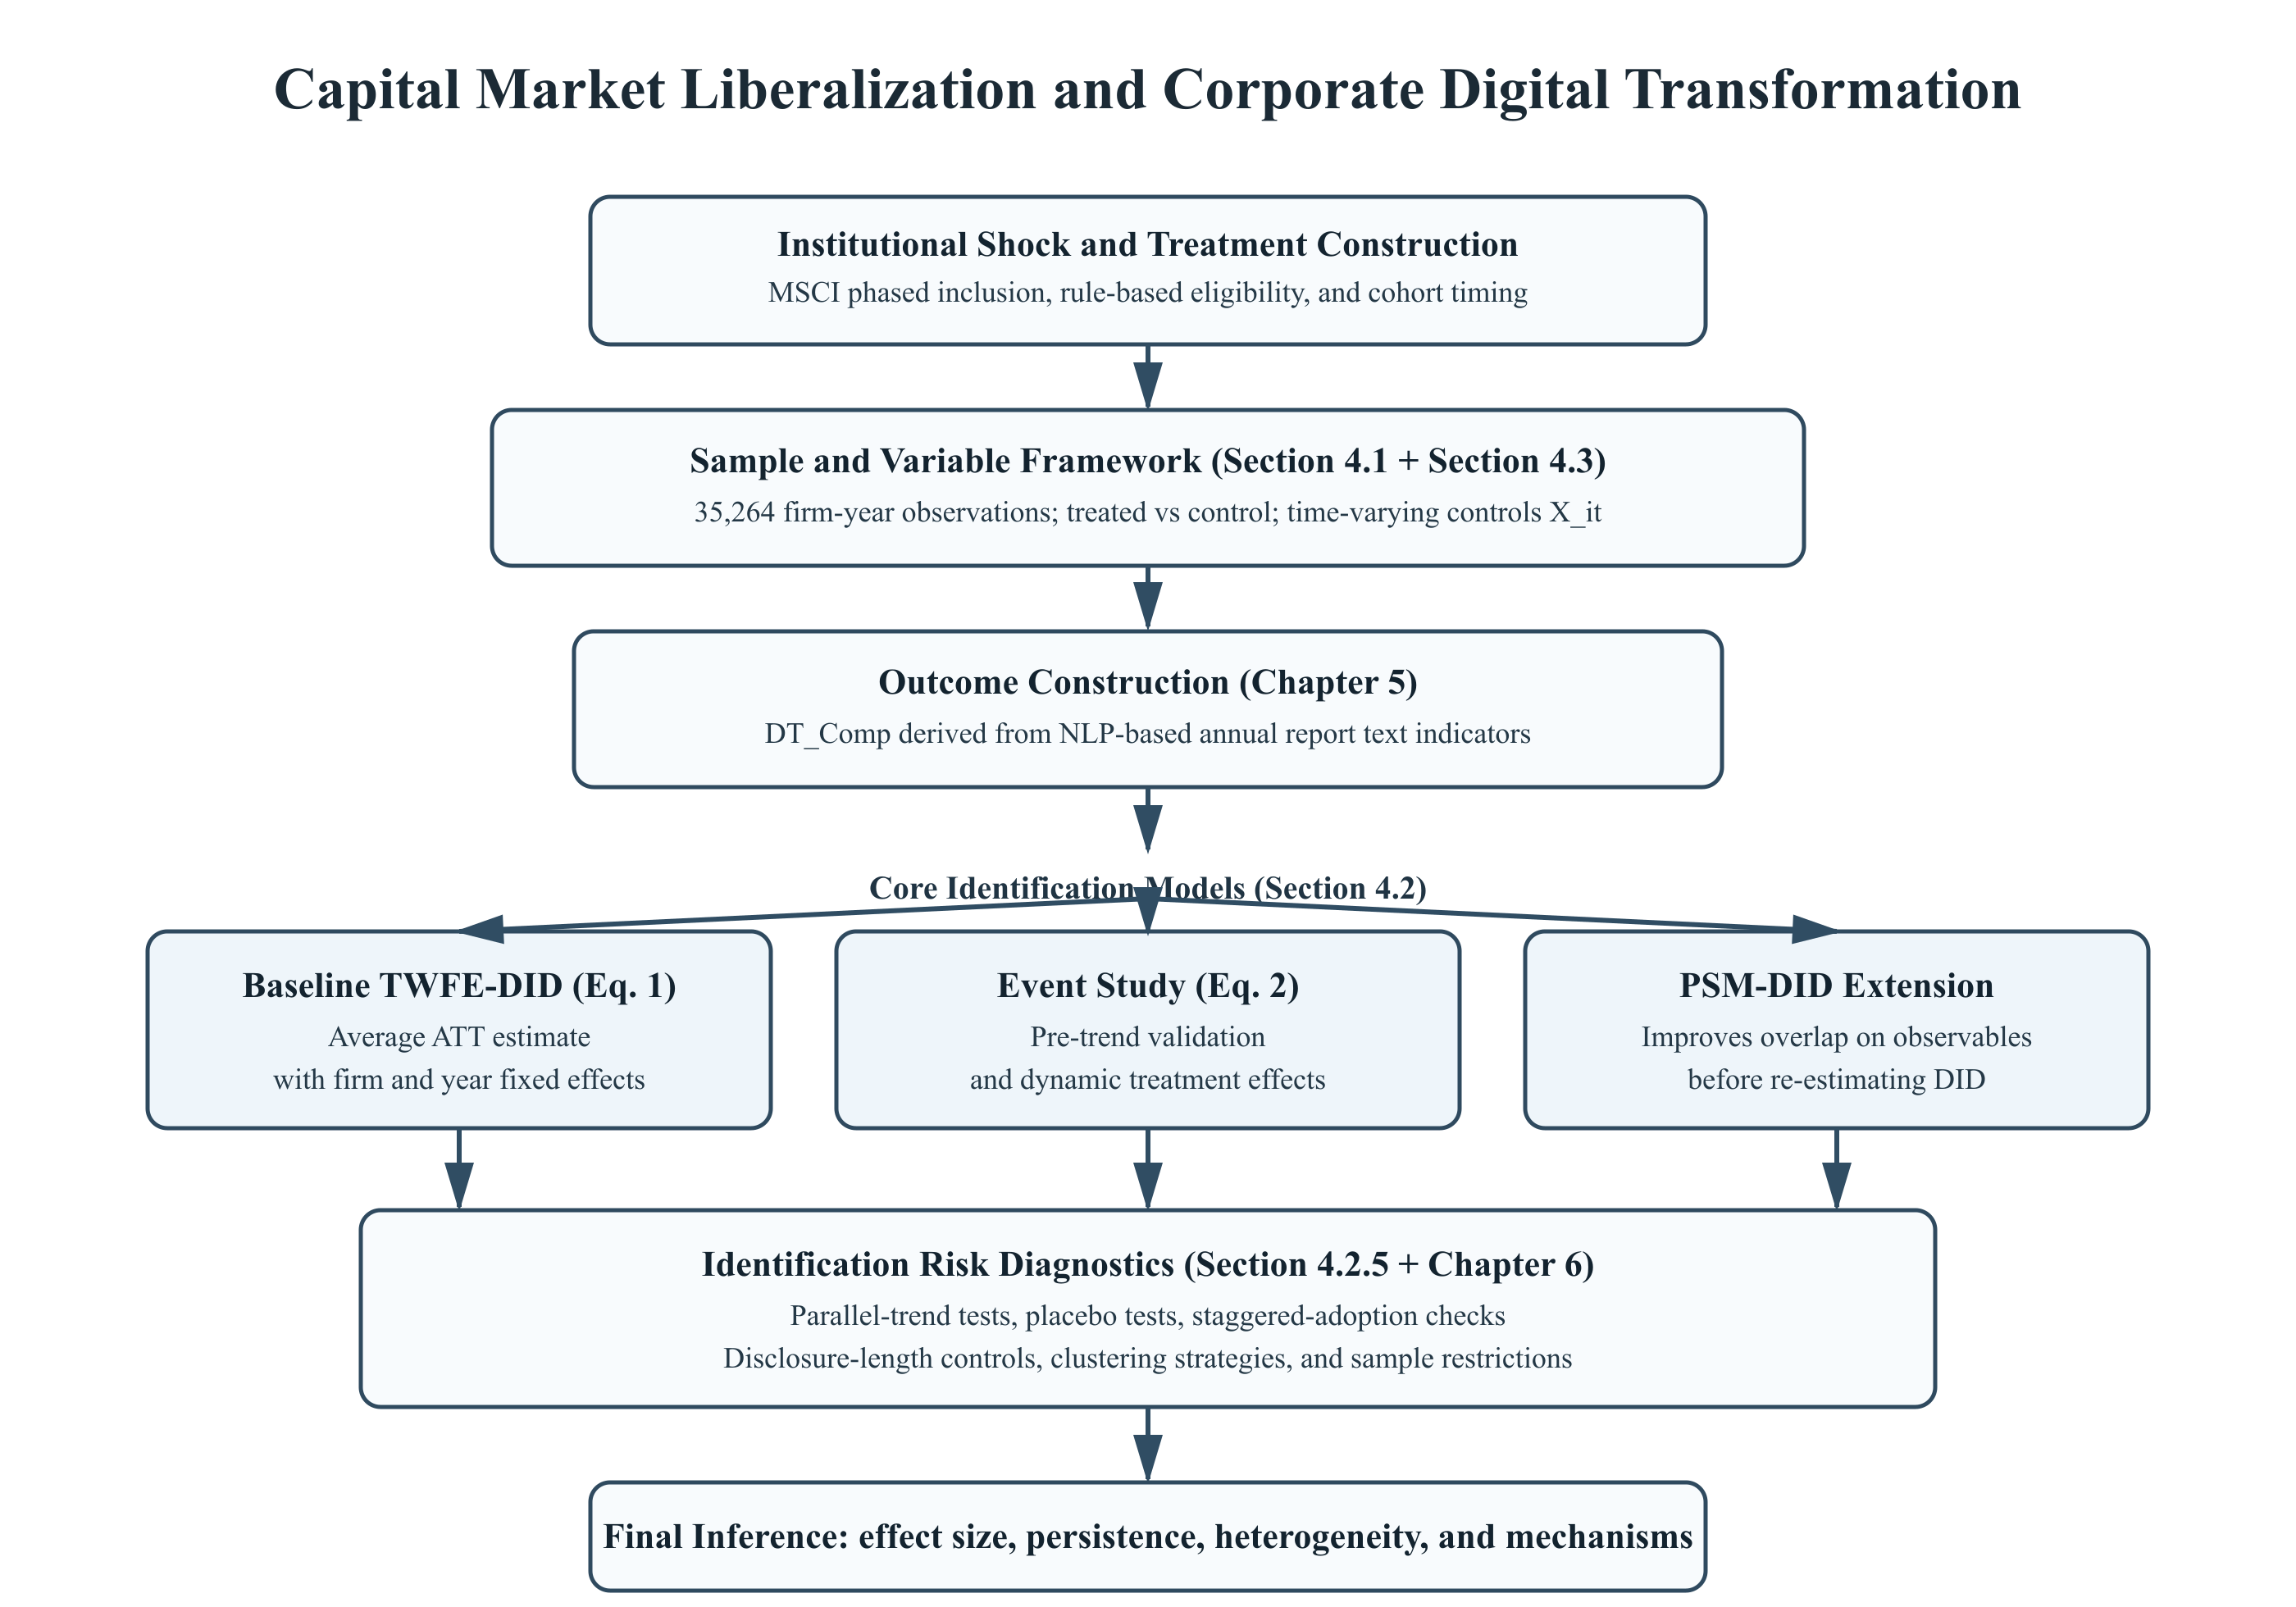
\includegraphics[width=0.92\textwidth]{figures/model_design_workflow.png}
\caption{Research Model Design Workflow}
\label{fig:model_design}
\end{figure}

As a research model design, Figure~\ref{fig:model_design} highlights the inferential logic of the chapter: causal identification does not rely on a single estimator, but on convergence across model structure, dynamic diagnostics, and robustness checks. This structure clarifies how each component contributes to internal validity and motivates the detailed specifications in Sections~\ref{sec:natural_experiment}--\ref{sec:threats}.

\subsection{The Natural Experiment: Exogeneity and Identification Logic}
\label{sec:natural_experiment}

MSCI inclusion meets the key requirements of a natural experiment. Inclusion criteria are mechanical---free-float market capitalization, liquidity thresholds, and Stock Connect accessibility---and are independent of firms' underlying digital transformation trajectories. The policy schedule was enforced externally by MSCI, without input from Chinese authorities or individual firms. These properties generate plausibly exogenous variation in international capital access, supporting the causal interpretation of our DID estimates. Following contemporary causal-design standards, we do not rely on exogeneity by assertion alone; instead, we combine institutional argumentation with empirical diagnostics, including pre-trend checks, placebo assignments, and alternative estimators designed for staggered treatment settings.

\subsection{Two-way fixed effects difference-in-differences specification}

We estimate the following two-way fixed effects DID specification:
\begin{equation}
\label{eq:twfe_did}
DT_{it} = \alpha + \beta\left(\mathrm{MSCI}_i \times \mathrm{Post}_t\right) + \gamma' X_{it} + \mu_i + \lambda_t + \varepsilon_{it}
\end{equation}
where $DT_{it}$ represents firm $i$'s digital transformation score in fiscal year $t$; $\mathrm{MSCI}_i$ equals one for constituent firms; $\mathrm{Post}_t$ equals one from 2018 onward; $X_{it}$ is a vector of time-varying control variables; $\mu_i$ and $\lambda_t$ capture firm and year fixed effects, respectively; and $\varepsilon_{it}$ is the idiosyncratic disturbance clustered at the firm level. The coefficient of interest, $\beta$, measures the average treatment effect on the treated.

\subsection{Event Study Design and Dynamic Treatment Indicators}

To analyze the temporal pattern of treatment effects and validate pre-treatment parallel trends, we estimate the event-study specification:
\begin{equation}
\label{eq:event_study}
DT_{it} = \alpha + \sum_{k} \delta_k \, \mathrm{MSCI}_i \times \mathbf{1}[t - T_i = k] + \gamma' X_{it} + \mu_i + \lambda_t + \varepsilon_{it}
\end{equation}
where $T_i$ denotes firm $i$'s inclusion year, and $k = -1$ is omitted as the reference period. Dynamic coefficients $\delta_k$ reveal whether digital transformation intensity rises precisely around the inclusion window and whether effects persist over time.

\subsection{Propensity score matching difference-in-differences (PSM-DID)}

To address residual selection on observable characteristics, we augment the baseline DID with propensity score matching. We estimate inclusion probability using pre-treatment (2016) characteristics via logistic regression, implement nearest-neighbor matching with replacement and a 0.01 caliper, and retain up to three controls per treated firm. Covariate balance diagnostics confirm standardized mean differences below 0.1 for all matching variables. Re-estimating Equation~(\ref{eq:twfe_did}) on the matched panel yields a PSM-DID estimator robust to observable selection bias. Methodologically, the matched design is used as a complement rather than a substitute for fixed-effects identification: matching improves overlap on observables, while DID continues to absorb time-invariant unobserved heterogeneity and common shocks.

\subsection{Threats to Identification and Mitigation Strategies}
\label{sec:threats}

The main identification threats are: (i)~pre-existing trends, where firms eventually selected into MSCI may already have had faster digital-transformation growth; (ii)~confounding events, where contemporaneous shocks (for example, STAR Market reforms or COVID-19) may affect treated and control firms differently; and (iii)~strategic disclosure responses, where post-inclusion language changes may not reflect operational change. We address these risks through event-study pre-trend tests, exclusions around major contemporaneous reforms, disclosure-length robustness checks, and 1,000-iteration placebo tests. We also report staggered-adoption diagnostics motivated by the modern DID literature, which shows that conventional TWFE estimates can be distorted under heterogeneous treatment effects. Taken together, these safeguards reduce the chance that results are driven by differential trends, timing artifacts, or pure disclosure inflation.

\section{Data Descriptions and Descriptive Statistics}

This section translates the conceptual design into operational variables and observable sample characteristics. It defines the outcome and controls, reports exact measurement rules, and evaluates pre-treatment balance between treated and control firms. These diagnostics provide the empirical context needed to interpret later regression estimates with appropriate caution and credibility.

\subsection{Variable Definition}

Precise variable definitions are essential for interpreting and replicating any empirical study in corporate finance. The analytical design used here combines a treatment indicator that captures access to international capital markets with a text-based outcome variable, a comprehensive set of financial controls, and governance proxies---each of which must be clearly defined before estimation. Treatment status is identified through a binary indicator for MSCI Emerging Markets Index constituents; the main outcome variable, digital transformation intensity, is built from natural language processing of mandatory annual reports, as described in Chapter~\ref{chap:research_design_2}; and the control variables include firm size, age, profitability ratios, leverage, cash flow, market valuation, ownership concentration, and board composition. All variables are based on established theory, and their selection follows prior practices in the literature on capital market liberalization and corporate digital transformation.

\begin{table}[htbp]
\centering
\caption{Variable Definitions}
\label{tab:variable_definitions}
\small
\begin{tabular}{lll}
\toprule
\textbf{Variable} & \textbf{Description} & \textbf{Unit} \\
\midrule
MSCI & Dummy = 1 if firm is in MSCI EM Index & Binary (0/1) \\
DT\_Comp\_A & DT degree based on annual report text mining & Word Count Index \\
Size & Natural logarithm of total assets (million RMB) & Log(Million CNY) \\
FirmAge & Years since firm incorporation & Years \\
ROA & Net income / Total assets & Ratio \\
ROE & Net income / Total shareholders' equity & Ratio \\
Leverage & Total liabilities / Total assets & Ratio \\
CashFlow & Operating cash flow / Total assets & Ratio \\
TobinQ & (MV equity + BV debt) / BV assets & Ratio \\
Ownership & Ownership \% of largest shareholder & Percentage (\%) \\
BoardSize & Number of board members & Count \\
IndepDir & Number of independent directors on the board & Count \\
\bottomrule
\end{tabular}
\begin{tablenotes}
\small
\item \textit{Notes:} All variables follow standard academic conventions. Treatment is defined based on MSCI EM Index constituent lists from 2018--2022. Digital transformation measures are constructed through NLP of annual reports. Financial variables are sourced from CSMAR database. All continuous variables are winsorized at 1st and 99th percentiles.
\end{tablenotes}
\end{table}

Table~\ref{tab:variable_definitions} provides formal definitions for all variables employed in the empirical analysis. The dependent variable, digital transformation intensity, is measured through NLP of annual reports, constructed as:
\begin{equation}
\label{eq:dt_comp}
DT\_Comp = \log\left(1 + \sum_{j} \mathrm{keywordsCount}_j\right)
\end{equation}
where $\mathrm{keywordsCount}_j$ denotes the frequency of keywords associated with technology domain $j$ across six digital technology clusters. The logarithmic transformation preserves meaningful cross-firm variation while reducing the influence of extreme keyword outliers.

The control vector $X_{it}$ includes:
\begin{equation}
\label{eq:control_vector}
\begin{aligned}
X_{it} = [&\log(\mathrm{asset}_{it}),\; \mathrm{Age}_{it},\; \mathrm{ROA}_{it},\; \mathrm{ROE}_{it},\; \mathrm{Leverage}_{it},\\
&\mathrm{CashFlow/Asset}_{it},\; Q_{it},\; \mathrm{OwnConc}_{it},\; \mathrm{BoardSize}_{it},\; \mathrm{IndepDirPct}_{it}]
\end{aligned}
\end{equation}
For mechanism analysis in Chapter~\ref{chap:empirical_results}, this baseline variable set is complemented by channel-specific outcomes. Direct knowledge-transfer mediators (analyst coverage and foreign institutional ownership) are conceptually preferred for mechanism identification, but they are not included in the current merged panel and are therefore reserved for future extensions.

All continuous variables are winsorized at the 1st and 99th percentiles to mitigate the influence of extreme observations.

\subsection{Measurement of Variables}

Reproducibility requires conceptual variables to map precisely to their computational counterparts in the source database. Small operational choices---for example, whether leverage uses total liabilities or net debt, or whether firm age is based on listing year versus incorporation year---can materially change coefficient magnitudes and significance. The measurement specifications below therefore document each technical field name, data type, and computational formula used in the analysis, aligned directly with CSMAR GTA column identifiers.

\begin{table}[htbp]
\centering
\caption{Variable Measurements}
\label{tab:variable_measurements}
\small
\begin{tabular}{llll}
\toprule
\textbf{Variable} & \textbf{Technical Name} & \textbf{Type} & \textbf{Calculation} \\
\midrule
MSCI & MSCI & Binary & = 1 if in MSCI EM Index \\
DT\_Comp\_A & dt\_transformation\_degree\_a & Cont. & DT keyword count \\
Size & size & Cont. & $\ln$(total assets in M RMB) \\
FirmAge & firm\_age & Cont. & Current year $-$ incorporation year \\
ROA & roa & Cont. & Net income / Total assets \\
ROE & roe & Cont. & Net income / Total equity \\
Leverage & Finlev & Cont. & Total liabilities / Total assets \\
CashFlow & cash & Cont. & Operating CF / Total assets \\
TobinQ & tobin & Cont. & (MV equity + BV debt) / BV assets \\
Ownership & top1 & Cont. & \% ownership of largest SH \\
BoardSize & BoardScale\_57 & Count & Total board directors \\
IndepDir & IndependentDirectorNumber1 & Count & Independent directors \\
\bottomrule
\end{tabular}
\begin{tablenotes}
\small
\item \textit{Notes:} Total variables: 12. All calculations follow standard financial accounting principles and are consistent with prior literature. Technical names (e.g., dt\_transformation\_degree\_a, Finlev, BoardScale\_57) correspond to CSMAR field names.
\end{tablenotes}
\end{table}

Table~\ref{tab:variable_measurements} documents the technical measurement specifications for each variable, including data types, computational formulas, and CSMAR database field mappings.

\subsection{Descriptive Statistics and Pre-Treatment Group Comparisons}

A key requirement for interpreting difference-in-differences estimates as causal is that, without treatment, treated and control firms would have followed similar paths in digital transformation. Pre-treatment covariate comparisons serve two main purposes: they identify whether the groups differ systematically on factors that could threaten this assumption, and they support the use of propensity score matching to achieve balance on observed variables. MSCI constituent selection is based on size, liquidity, and accessibility criteria, which means treated firms are likely to differ from typical A-share controls in meaningful ways related to organizational capacity for technology adoption. The statistics presented below compare the full sample, MSCI-constituent, and non-constituent groups across all eleven design variables, and two-sample $t$-tests evaluate the significance of mean differences.

\begin{table}[htbp]
\centering
\caption{Descriptive Statistics}
\label{tab:descriptive_stats}
\scriptsize
\resizebox{\textwidth}{!}{%
\begin{tabular}{lccccccc}
\toprule
\textbf{Variable} & \textbf{Full Mean} & \textbf{Full SD} & \textbf{MSCI Mean} & \textbf{MSCI SD} & \textbf{Non-MSCI Mean} & \textbf{Non-MSCI SD} & \textbf{Diff ($t$-stat)} \\
\midrule
Digital Transformation & 12.98 & 33.14 & 22.21 & 46.39 & 12.78 & 33.30 & 9.44*** (10.95) \\
Firm Size (log) & 22.14 & 1.30 & 24.34 & 1.28 & 22.03 & 1.20 & 2.31*** (76.03) \\
Firm Age & 9.70 & 7.62 & 15.55 & 7.17 & 9.42 & 7.52 & 6.14*** (32.35) \\
ROA & 0.036 & 0.099 & 0.063 & 0.069 & 0.035 & 0.100 & 0.028*** (11.35) \\
ROE & 0.009 & 1.988 & 0.103 & 0.148 & 0.004 & 2.036 & 0.099** (1.98) \\
Leverage & 0.401 & 0.257 & 0.421 & 0.246 & 0.400 & 0.257 & 0.021*** (3.29) \\
CashFlow & 0.213 & 0.155 & 0.212 & 0.141 & 0.213 & 0.155 & $-$0.002 ($-$0.40) \\
Tobin's Q & 2.164 & 4.637 & 2.549 & 2.552 & 2.146 & 4.714 & 0.404*** (3.45) \\
Ownership Conc. & 34.17 & 14.94 & 36.42 & 15.68 & 34.06 & 14.90 & 2.37*** (6.27) \\
Board Size & 6.89 & 3.27 & 8.25 & 2.93 & 6.83 & 3.27 & 1.43*** (17.33) \\
Indep.\ Directors & 3.16 & 0.57 & 3.44 & 0.76 & 3.15 & 0.56 & 0.30*** (20.67) \\
Observations & \multicolumn{2}{c}{35,264} & \multicolumn{2}{c}{1,644} & \multicolumn{2}{c}{33,620} & \\
\bottomrule
\end{tabular}
}
\begin{tablenotes}
\small
\item \textit{Notes:} Sample spans 2010--2022. MSCI firms are those included starting 2018. All continuous variables are winsorized at 1st and 99th percentiles. $t$-statistics from two-sample $t$-tests in parentheses. Significance: *** $p < 0.01$, ** $p < 0.05$, * $p < 0.10$. The large $N$ differential (1,644 treated vs.\ 33,620 control) reflects MSCI's selective mechanical criteria.
\end{tablenotes}
\end{table}

Table~\ref{tab:descriptive_stats} presents comprehensive descriptive statistics for the full sample and separately for MSCI constituent and non-constituent firms. Several patterns emerge.

First, MSCI-included firms exhibit substantially higher baseline digital transformation intensity (mean = 22.21 keyword counts) compared to non-included firms (mean = 12.78), a difference of 9.44 that is statistically significant at the 1\% level ($t = 10.95$). Second, treated firms are systematically larger, with mean log assets of 24.34 versus 22.03 for controls, corresponding to approximately a 10-fold difference in asset scale. Third, MSCI constituents are more mature, averaging 15.6 years since incorporation versus 9.4 years for non-constituents. Fourth, treated firms demonstrate superior financial performance: higher profitability (ROA: 6.3\% vs.\ 3.5\%), stronger equity returns (ROE: 10.3\% vs.\ 0.4\%), and elevated market valuations (Tobin's $Q$: 2.55 vs.\ 2.15). Fifth, governance structures differ systematically, with MSCI firms maintaining larger boards and more independent directors. Interestingly, financial leverage (42.1\% vs.\ 40.0\%) and cash flow ratios (21.2\% vs.\ 21.3\%) are economically similar across groups.

These systematic pre-treatment differences underscore the importance of our combined DID and PSM identification strategy.

Chapter~\ref{chap:research_design_2} then documents construction and validation of the text-based outcome variables, and Chapter~\ref{chap:empirical_results} implements the estimation sequence defined in this chapter.
